\section{数据集、评价指标与方法方案}\label{sec:method}

\subsection{章节说明}

这一章先把实验前置条件说清楚，包括数据集来源、预处理方式、评价指标、模型选择和实验口径。由于后续同时涉及 MMDetection、Ultralytics 和本地模型插件，数据与结果如果不先对齐，表格中的数值就很难横向解释。因此，这里不只列出“用了什么”，也交代这些设置为什么会影响后面的分析。

\subsection{数据集介绍}

实验采用 LEVIR-Ship 数据集作为统一基准\cite{chen2022_tinyship_drenet}。该数据集面向中分辨率遥感微小船舶检测任务，能够反映复杂海面背景下小目标检出的实际难点。数据集划分见表~\ref{tab:ch3_dataset_split}。

\begin{table}[htbp]
  \centering
  \caption{LEVIR-Ship 数据集划分}
  \label{tab:ch3_dataset_split}
  \begin{tabular}{lcc}
    \toprule
    数据子集 & 图像数量 & 目标数量 \\
    \midrule
    训练集 & 2321 & 2002 \\
    验证集 & 788 & 665 \\
    测试集 & 788 & 552 \\
    \bottomrule
  \end{tabular}
\end{table}

LEVIR-Ship 中的船舶目标普遍较小，背景又不干净。部分图像中，船体与海浪、岸线或港区设施的局部纹理差异并不明显；当输入尺寸变化或后处理阈值调整时，模型输出也会随之改变。基于这些观察，本文在实验设计中同时记录检出能力、误检控制和工程部署相关指标，而不是只依赖一个主指标判断模型优劣。

\subsection{数据集样例与任务特征}

LEVIR-Ship 覆盖开阔海域、近岸区域、港口区域和多目标密集分布等场景，不同图像块在背景纹理、目标密度、目标朝向和局部对比度上差异较大。这意味着模型既要对微弱目标保持敏感，也要抑制复杂背景中的伪目标响应。对遥感微小船舶检测而言，“目标小而背景强”正是任务难点的集中体现。

\begin{figure}[htbp]
  \centering
  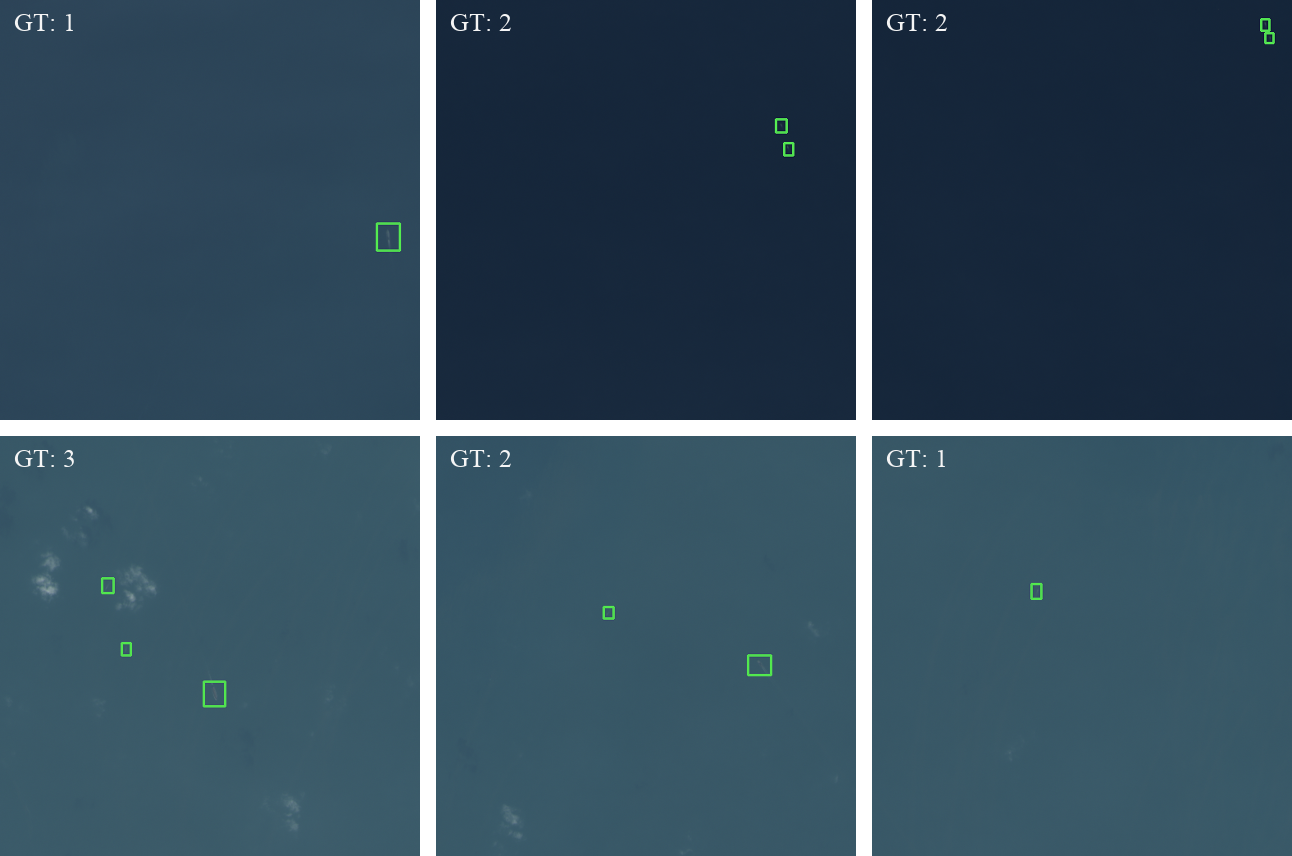
\includegraphics[width=0.88\textwidth]{img/ch3_dataset_examples.png}
  \caption{LEVIR-Ship 数据集典型样例}
  \label{fig:ch3_dataset_examples}
\end{figure}

考虑到这些场景差异，后续实验除 AP50 外，还会记录 Precision、Recall、F1，并保留成功检测、漏检和误检样例。这样可以把“分数高低”和“具体错在哪里”放在一起看。对同时包含实验和系统实现的课题而言，这一点比单独追求一个精度值更重要。

\subsection{数据预处理与统一格式}

跨框架实验里，最容易出偏差的地方往往不是网络结构，而是数据和评测脚本。为把这部分误差压下去，实验前先统一数据预处理和结果组织方式。

处理流程分为几步。第一步核对图像和标注文件是否一一对应，并检查空标注、异常坐标和类别不一致等情况。第二步将数据整理为 COCO 中间格式，使 MMDetection 路线和 YOLO 路线尽量共享同一评测基础。第三步固定 train、val、test 划分及样本清单，避免模型之间因为样本范围不同而产生额外差异。最后，各模型输出统一整理为包含 \texttt{image\_id}、\texttt{model\_name}、\texttt{bbox}、\texttt{score} 和 \texttt{category\_id} 的结构化记录，供可视化和数据库存储复用。

这些处理的用意很直接：尽量让差异来自检测范式和实现策略，而不是来自数据组织或脚本细节。若每个模型都使用不同划分、不同评测脚本和不同输出字段，后续得到的数值就很难解释。统一格式和统一口径在本文中属于实验方法的一部分，不只是训练前的文件整理。

统一格式也直接服务于系统实现。MMDetection、YOLO 和本地插件的推理结果可以进入同一套后处理与可视化逻辑，跨框架联调成本会低一些；结构化结果也能写入 Web 系统数据库，使离线实验结果和在线任务回放使用同一类数据表达。

\subsection{评价指标}

实验采用 AP50 作为主指标，并以 AP50-95、Precision、Recall 与 F1 作为辅助指标。相关定义如下。

\begin{equation}
\text{Precision} = \frac{TP}{TP + FP}
\end{equation}

\begin{equation}
\text{Recall} = \frac{TP}{TP + FN}
\end{equation}

\begin{equation}
F1 = \frac{2 \cdot \text{Precision} \cdot \text{Recall}}{\text{Precision} + \text{Recall}}
\end{equation}

\begin{equation}
\text{IoU} = \frac{|B_{pred} \cap B_{gt}|}{|B_{pred} \cup B_{gt}|}
\end{equation}

其中，AP50 对应 IoU 阈值为 0.5 时的平均精度，本文用它观察模型是否能把微小船舶找出来；AP50-95 覆盖多个 IoU 阈值，对边框位置质量更敏感；Precision 更接近误检控制情况，Recall 更接近漏检控制情况，F1 用于观察二者折中。本文还记录 FPS、参数量和 FLOPs，用于讨论模型接入系统时的部署成本。

\subsection{指标选择依据}

AP50 放在主指标位置，主要是因为船舶目标太小。预测框和标注框只要偏移几个像素，IoU 就可能明显变化。若过度依赖高 IoU 阈值，边框回归误差会被放大，“模型是否发现目标”反而看不清楚。AP50 用来回答基本检出能力，AP50-95 则补充观察定位质量。

Precision、Recall 和 F1 在本文中同样重要。DRENet、FCOS 与 YOLO26 的设计出发点不同，只按 AP50 排序，容易掩盖误检和漏检之间的取舍。Recall 高的模型适合目标排查类场景，Precision 高的模型更适合输出需要稳定可控的系统展示场景。后续分析会把 Precision--Recall 平衡作为解释模型行为的主要依据之一。

\subsection{模型方案}

为了让对比不局限在同一类检测器内部，本文选取三类模型：DRENet 对应遥感微小船舶专项方法，FCOS 对应 anchor-free 参考路线，YOLO26 对应 one-stage 轻量部署路线。

\subsubsection{DRENet（专项方法）}

DRENet 是针对 LEVIR-Ship 场景提出的专项方法\cite{chen2022_tinyship_drenet}。它在训练阶段引入退化重建增强机制，试图让网络更关注弱纹理船舶目标。本文将 DRENet 作为主线模型之一，重点观察它在 Recall、复杂背景和召回优先任务中的表现。

\begin{figure}[htbp]
  \centering
  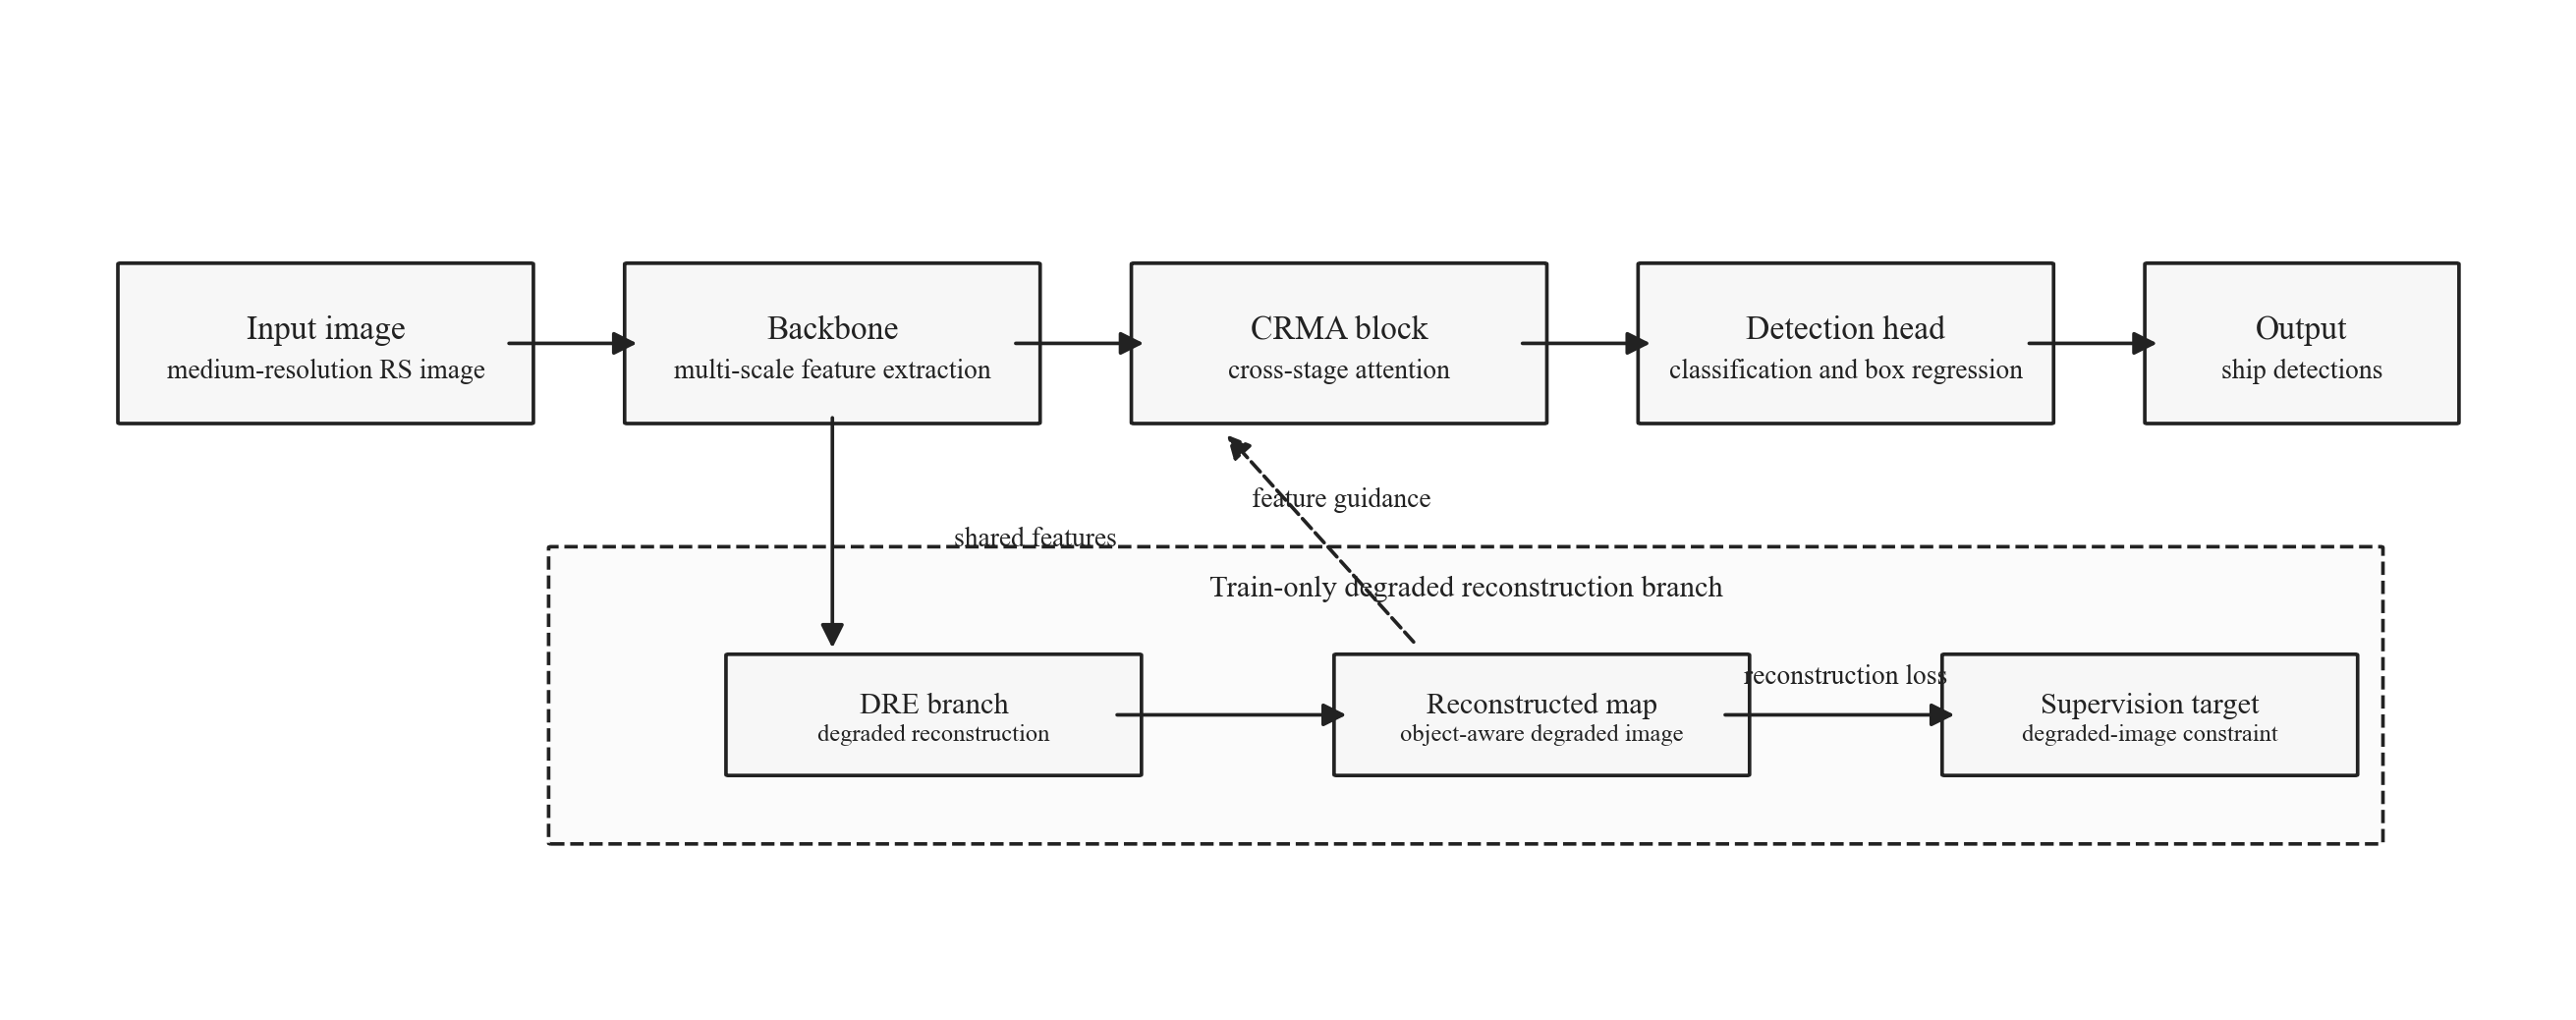
\includegraphics[width=0.95\textwidth]{img/ch3_drenet_overview.png}
  \caption{DRENet 方法示意}
  \label{fig:ch3_drenet_overview}
\end{figure}

图~\ref{fig:ch3_drenet_overview} 中可以看到，DRENet 在常规检测路径外加入了退化重建增强分支。该分支只参与训练，通过重建带有目标感知信息的退化图像约束骨干网络特征，使模型减少对大面积背景纹理的依赖。结合 CRMA 模块的跨阶段特征增强设计，DRENet 在本文实验中表现出比较明显的召回优先倾向。

\subsubsection{FCOS（Anchor-Free 参考基线）}

FCOS 用位置回归替代锚框设计，减少了 anchor 尺寸、比例和匹配策略等超参数依赖\cite{tian2019_fcos}。在本文中，它更多承担 anchor-free 参照基线的角色，用来观察不加入遥感专项结构时，通用 anchor-free 检测器在该任务上的表现。需要说明的是，当前可回填的 FCOS 正式结果来自 MMDetection 默认输入策略，因此本文只把它作为参考和补充比较对象，不把它放入严格同输入尺度的主结论竞争。

\begin{figure}[htbp]
  \centering
  
\includegraphics[width=0.95\textwidth]{img/ch3_fcos_pipeline.png}
  \caption{FCOS 检测流程示意}
  \label{fig:ch3_fcos_pipeline}
\end{figure}

图~\ref{fig:ch3_fcos_pipeline} 展示了 FCOS 的基本流程。输入图像经过 Backbone 和 FPN 后生成多尺度特征，检测头直接预测类别、边框偏移和 centerness 分数。由于没有显式 anchor 设计，FCOS 适合作为本文的 anchor-free 对照。

\subsubsection{YOLO26（One-Stage 轻量部署代表）}

YOLO 系列以单阶段预测和推理效率见长，在工程部署中使用较多\cite{redmon2016_yolo,redmon2018_yolov3,ultralytics2024_docs}。本文选取 YOLO26 代表 one-stage 路线，关注它在检测精度、边框质量、训练链路成熟度和系统接入成本之间的表现。

\begin{figure}[htbp]
  \centering
  
\includegraphics[width=0.95\textwidth]{img/ch3_yolo_pipeline.png}
  \caption{YOLO26 单阶段检测流程示意}
  \label{fig:ch3_yolo_pipeline}
\end{figure}

如图~\ref{fig:ch3_yolo_pipeline} 所示，YOLO26 延续了典型 one-stage 结构：Backbone 提取特征，Neck 做多尺度融合，检测头一次输出候选框。相较于专项结构较多的模型，它在训练、部署和接口封装上更直接，因此适合作为系统默认模型的候选。

\subsection{统一实验协议与实现约束}

为了让后续比较有明确边界，本文对实验协议作了几项约束：数据划分和评测口径保持一致；DRENet 与 YOLO26 的主线实验统一采用 512 输入；FCOS 标注为历史正式结果对应的 anchor-free 参考基线，并在文中说明输入尺度差异；实验环境、配置文件、权重路径、日志文件和关键结果都保留记录；结果输出结构也统一整理，便于系统侧复用。

需要强调的是，统一协议并不等于把所有模型改造成完全相同的实现。本文保留客观实现边界，并在对应章节说明。比如，FCOS 当前正式结果来自 MMDetection 默认输入策略，所以只作为参考基线；DRENet 在本地插件路径下使用非 512 输入会触发 shape mismatch，因此尺寸敏感性分析中不强行补齐 640 和 800 的结果。这个处理偏保守，但能保证论文描述和实际实现一致。

在实现层面，本文通过统一推理入口封装不同模型能力：

\begin{verbatim}
predict(image_path, model_name, conf_threshold, iou_threshold)
\end{verbatim}

在此基础上，本文继续封装融合推理接口和系统任务执行逻辑。模型训练后的离线评测、命令行单图推理、批量推理以及 Web 系统接入，都尽量复用同一个核心入口。这样既减少重复代码，也便于核对离线结果和系统展示结果是否来自同一套推理逻辑。

\subsection{小结}

到这里，数据集、预处理流程、评价指标、模型选择和实验协议已经固定下来。后续实验结果、误差分析和系统实现都在这套数据与接口基础上展开。
